% Options for packages loaded elsewhere
\PassOptionsToPackage{unicode}{hyperref}
\PassOptionsToPackage{hyphens}{url}
%
\documentclass[
]{book}
\usepackage{amsmath,amssymb}
\usepackage{lmodern}
\usepackage{iftex}
\ifPDFTeX
  \usepackage[T1]{fontenc}
  \usepackage[utf8]{inputenc}
  \usepackage{textcomp} % provide euro and other symbols
\else % if luatex or xetex
  \usepackage{unicode-math}
  \defaultfontfeatures{Scale=MatchLowercase}
  \defaultfontfeatures[\rmfamily]{Ligatures=TeX,Scale=1}
\fi
% Use upquote if available, for straight quotes in verbatim environments
\IfFileExists{upquote.sty}{\usepackage{upquote}}{}
\IfFileExists{microtype.sty}{% use microtype if available
  \usepackage[]{microtype}
  \UseMicrotypeSet[protrusion]{basicmath} % disable protrusion for tt fonts
}{}
\makeatletter
\@ifundefined{KOMAClassName}{% if non-KOMA class
  \IfFileExists{parskip.sty}{%
    \usepackage{parskip}
  }{% else
    \setlength{\parindent}{0pt}
    \setlength{\parskip}{6pt plus 2pt minus 1pt}}
}{% if KOMA class
  \KOMAoptions{parskip=half}}
\makeatother
\usepackage{xcolor}
\usepackage{color}
\usepackage{fancyvrb}
\newcommand{\VerbBar}{|}
\newcommand{\VERB}{\Verb[commandchars=\\\{\}]}
\DefineVerbatimEnvironment{Highlighting}{Verbatim}{commandchars=\\\{\}}
% Add ',fontsize=\small' for more characters per line
\usepackage{framed}
\definecolor{shadecolor}{RGB}{248,248,248}
\newenvironment{Shaded}{\begin{snugshade}}{\end{snugshade}}
\newcommand{\AlertTok}[1]{\textcolor[rgb]{0.94,0.16,0.16}{#1}}
\newcommand{\AnnotationTok}[1]{\textcolor[rgb]{0.56,0.35,0.01}{\textbf{\textit{#1}}}}
\newcommand{\AttributeTok}[1]{\textcolor[rgb]{0.77,0.63,0.00}{#1}}
\newcommand{\BaseNTok}[1]{\textcolor[rgb]{0.00,0.00,0.81}{#1}}
\newcommand{\BuiltInTok}[1]{#1}
\newcommand{\CharTok}[1]{\textcolor[rgb]{0.31,0.60,0.02}{#1}}
\newcommand{\CommentTok}[1]{\textcolor[rgb]{0.56,0.35,0.01}{\textit{#1}}}
\newcommand{\CommentVarTok}[1]{\textcolor[rgb]{0.56,0.35,0.01}{\textbf{\textit{#1}}}}
\newcommand{\ConstantTok}[1]{\textcolor[rgb]{0.00,0.00,0.00}{#1}}
\newcommand{\ControlFlowTok}[1]{\textcolor[rgb]{0.13,0.29,0.53}{\textbf{#1}}}
\newcommand{\DataTypeTok}[1]{\textcolor[rgb]{0.13,0.29,0.53}{#1}}
\newcommand{\DecValTok}[1]{\textcolor[rgb]{0.00,0.00,0.81}{#1}}
\newcommand{\DocumentationTok}[1]{\textcolor[rgb]{0.56,0.35,0.01}{\textbf{\textit{#1}}}}
\newcommand{\ErrorTok}[1]{\textcolor[rgb]{0.64,0.00,0.00}{\textbf{#1}}}
\newcommand{\ExtensionTok}[1]{#1}
\newcommand{\FloatTok}[1]{\textcolor[rgb]{0.00,0.00,0.81}{#1}}
\newcommand{\FunctionTok}[1]{\textcolor[rgb]{0.00,0.00,0.00}{#1}}
\newcommand{\ImportTok}[1]{#1}
\newcommand{\InformationTok}[1]{\textcolor[rgb]{0.56,0.35,0.01}{\textbf{\textit{#1}}}}
\newcommand{\KeywordTok}[1]{\textcolor[rgb]{0.13,0.29,0.53}{\textbf{#1}}}
\newcommand{\NormalTok}[1]{#1}
\newcommand{\OperatorTok}[1]{\textcolor[rgb]{0.81,0.36,0.00}{\textbf{#1}}}
\newcommand{\OtherTok}[1]{\textcolor[rgb]{0.56,0.35,0.01}{#1}}
\newcommand{\PreprocessorTok}[1]{\textcolor[rgb]{0.56,0.35,0.01}{\textit{#1}}}
\newcommand{\RegionMarkerTok}[1]{#1}
\newcommand{\SpecialCharTok}[1]{\textcolor[rgb]{0.00,0.00,0.00}{#1}}
\newcommand{\SpecialStringTok}[1]{\textcolor[rgb]{0.31,0.60,0.02}{#1}}
\newcommand{\StringTok}[1]{\textcolor[rgb]{0.31,0.60,0.02}{#1}}
\newcommand{\VariableTok}[1]{\textcolor[rgb]{0.00,0.00,0.00}{#1}}
\newcommand{\VerbatimStringTok}[1]{\textcolor[rgb]{0.31,0.60,0.02}{#1}}
\newcommand{\WarningTok}[1]{\textcolor[rgb]{0.56,0.35,0.01}{\textbf{\textit{#1}}}}
\usepackage{longtable,booktabs,array}
\usepackage{calc} % for calculating minipage widths
% Correct order of tables after \paragraph or \subparagraph
\usepackage{etoolbox}
\makeatletter
\patchcmd\longtable{\par}{\if@noskipsec\mbox{}\fi\par}{}{}
\makeatother
% Allow footnotes in longtable head/foot
\IfFileExists{footnotehyper.sty}{\usepackage{footnotehyper}}{\usepackage{footnote}}
\makesavenoteenv{longtable}
\usepackage{graphicx}
\makeatletter
\def\maxwidth{\ifdim\Gin@nat@width>\linewidth\linewidth\else\Gin@nat@width\fi}
\def\maxheight{\ifdim\Gin@nat@height>\textheight\textheight\else\Gin@nat@height\fi}
\makeatother
% Scale images if necessary, so that they will not overflow the page
% margins by default, and it is still possible to overwrite the defaults
% using explicit options in \includegraphics[width, height, ...]{}
\setkeys{Gin}{width=\maxwidth,height=\maxheight,keepaspectratio}
% Set default figure placement to htbp
\makeatletter
\def\fps@figure{htbp}
\makeatother
\setlength{\emergencystretch}{3em} % prevent overfull lines
\providecommand{\tightlist}{%
  \setlength{\itemsep}{0pt}\setlength{\parskip}{0pt}}
\setcounter{secnumdepth}{5}
\usepackage{booktabs}
\ifLuaTeX
  \usepackage{selnolig}  % disable illegal ligatures
\fi
\usepackage[]{natbib}
\bibliographystyle{plainnat}
\IfFileExists{bookmark.sty}{\usepackage{bookmark}}{\usepackage{hyperref}}
\IfFileExists{xurl.sty}{\usepackage{xurl}}{} % add URL line breaks if available
\urlstyle{same} % disable monospaced font for URLs
\hypersetup{
  pdftitle={Konzepte des Prozeduralen Programmierens},
  pdfauthor={Prof.~Dr.~Sascha Frohwerk},
  hidelinks,
  pdfcreator={LaTeX via pandoc}}

\title{Konzepte des Prozeduralen Programmierens}
\author{Prof.~Dr.~Sascha Frohwerk}
\date{2023-09-11}

\begin{document}
\maketitle

{
\setcounter{tocdepth}{1}
\tableofcontents
}
\hypertarget{vorwort}{%
\chapter*{Vorwort}\label{vorwort}}
\addcontentsline{toc}{chapter}{Vorwort}

Dies ist das Skript mit Beispielen und kurzen Erklärungen zur Vorlesung ``Konzepte des prozeduralen Programmierens'' an der FOM in Leipzig im Wintersemester 2023 / 2024. Weil das Skript aktuell aus einem anderen Format übertragen und dabei auch überarbeitet wird, liegt es noch nicht vollständig vor. Es wird sich während des Semsters weiterentwickeln und ist dann rechtzeitig vor der Klausur fertig sein.

\begin{center}\rule{0.5\linewidth}{0.5pt}\end{center}

\hypertarget{einleitung}{%
\chapter{Einleitung}\label{einleitung}}

-\textgreater{} siehe Folien

\begin{center}\rule{0.5\linewidth}{0.5pt}\end{center}

\hypertarget{Eingabe-Ausgabe-Operatoren}{%
\chapter{Eingabe, Ausgabe und einfache Operatoren}\label{Eingabe-Ausgabe-Operatoren}}

\hypertarget{hallo-eva}{%
\section{Hallo EVA}\label{hallo-eva}}

Bei einfachen Programmen sollte man sich (wenn möglich) an das EVA-Prinzip halten. Das erhöht die Lesbarkeit und macht die weitere Bearbeitung des Programms einfacher.

\begin{figure}
\centering
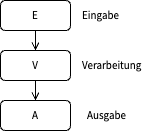
\includegraphics{assets/eva.png}
\caption{Das EVA-Prinzip}
\end{figure}

Der folgende Code zeigt ein einfaches Programm, das den Benutzer um die Eingabe einer ganzen Zahl bittet, diese mit zwei multipliziert und wieder ausgibt. Das Programm folgt dem EVA-Prinzip: Eingabe - Verarbeitung - Ausgabe. Dies hilft Code zu strukturieren und wir wollen versuchen, diesem Prinzip zu folgen, wenn es möglich ist.

\begin{verbatim}
# Eingabe
eingabe = input("Bitte eine Zahl eingeben:")

# Verarbeitung
zahl = int(eingabe)
ausgabe = 2*zahl

# Ausgabe
print(ausgabe)
\end{verbatim}

Anmerkungen dazu:

\begin{itemize}
\item
  Anweisungen werden von oben nach unten abgearbeitet
\item
  ``='' weist einer Variablen einen Wert zu
\item
  In Python müssen diese Variablen vorher nicht definiert werden
\item
  input() liest Werte ein
\item
  print() gibt Werte aus
\item
  int() wandelt einen String in einen Integer um
\item
  Zeilen mit einer Raute am Anfang sind Kommentare. Sie werden nicht übersetzt.
\end{itemize}

Die Namen von Variablen oder Funktionen nennen wir Bezeichner, hier z.B. ``eingabe''. Diese dürfen in Python mit einem Buchstaben oder einen Unterstrich beginnen (letzteres ist aber nicht zu empfehlen), aber nicht mit einer Zahl oder einem Sonderzeichen. Sie dürfen ausserdem nicht den Namen eines Schlüsselwortes haben. Schlüsselworte sind Worte, die in Python eine besondere Bedeutung haben, z.B. dürfen Sie Ihre Variable nicht ``while'' nennen, weil damit eine Schleife eingeleitet wird.

\hypertarget{weitere-tips-zum-umgang-mit-code}{%
\subsection*{Weitere Tips zum Umgang mit Code}\label{weitere-tips-zum-umgang-mit-code}}
\addcontentsline{toc}{subsection}{Weitere Tips zum Umgang mit Code}

Anweisungen in einer Zeile zusammenfassen:

\begin{Shaded}
\begin{Highlighting}[]
\NormalTok{a }\OperatorTok{=} \DecValTok{3}\OperatorTok{;}\NormalTok{ b }\OperatorTok{=} \DecValTok{6}\OperatorTok{;}
\BuiltInTok{print}\NormalTok{(a}\OperatorTok{+}\NormalTok{b)}
\end{Highlighting}
\end{Shaded}

\begin{verbatim}
## 9
\end{verbatim}

Lange Zeilen umbrechen:

\begin{Shaded}
\begin{Highlighting}[]
\NormalTok{a }\OperatorTok{=} \OperatorTok{\textbackslash{}}
\DecValTok{5}
\BuiltInTok{print}\NormalTok{(a)}
\end{Highlighting}
\end{Shaded}

\begin{verbatim}
## 5
\end{verbatim}

Ein- und Ausgabe von Zeichenketten (Strings):

\begin{Shaded}
\begin{Highlighting}[]
\BuiltInTok{print}\NormalTok{(}\StringTok{"Dein Name:"}\NormalTok{)}
\NormalTok{name }\OperatorTok{=} \BuiltInTok{input}\NormalTok{()}
\BuiltInTok{print}\NormalTok{(}\StringTok{"Hallo "}\OperatorTok{+}\NormalTok{name)}
\end{Highlighting}
\end{Shaded}

Seit Python 3.6 gibt eine weitere Möglichkeit Strings und andere Variablen zu verknüpfen: f-Strings

\begin{Shaded}
\begin{Highlighting}[]
\NormalTok{name }\OperatorTok{=} \StringTok{"Klaus"}
\BuiltInTok{print}\NormalTok{(}\SpecialStringTok{f"Hallo }\SpecialCharTok{\{}\NormalTok{name}\SpecialCharTok{\}}\SpecialStringTok{"}\NormalTok{)}
\end{Highlighting}
\end{Shaded}

\begin{verbatim}
## Hallo Klaus
\end{verbatim}

\hypertarget{einfache-datentypen}{%
\section{Einfache Datentypen}\label{einfache-datentypen}}

Man unterscheidet zwischen einfachen und strukturierten Datentypen. Einfache Datentypen können eine einzige Information, zum Beispiel eine Zahl, speichern. Strukturierte Datentypen können mehrere Zusammenhänge Daten speichern. Hierbei kann es sich zum Beispiel um Listen oder Tabellen handeln. Die folgende Abbildung gibt einen Überblick über die in Python vorhandenen Datentypen.

\hypertarget{datentypen-allgemein}{%
\subsection*{Datentypen allgemein}\label{datentypen-allgemein}}
\addcontentsline{toc}{subsection}{Datentypen allgemein}

In allen Programmiersprachen und Datenbanksystemen gibt es Datentypen. Sie definieren, welche Art von Daten eine Variable oder eine Spalte in einer Tabelle aufnehmen kann. Allgemein gibt es folgende grundlegende Datentypen:

\begin{longtable}[]{@{}llll@{}}
\caption{Datentypen allgemein}\tabularnewline
\toprule()
Typ & Python & C & MySQL \\
\midrule()
\endfirsthead
\toprule()
Typ & Python & C & MySQL \\
\midrule()
\endhead
nichts & None & null, void & null \\
ganze Zahlen & int & int & int \\
Fließkommazahlen & float & float, double & float \\
komplexe Zahlen & complex & float complex & - \\
Buchstaben & bytearray & char & char \\
Zeichenketten & string & - & varchar \\
Wahrheitswerte & bool & - & boolean \\
\bottomrule()
\end{longtable}

In C gibt es nativ keinen Datentyp für Wahrheitswerte. Dies wird über die Integer-Werte 0 (falsch) und 1 (wahr) ausgedrückt. Seit C99 gibt es \_Bool und bool. Es gibt von jedem Grundtyp noch mehrere Varianten in Abhängigkeit von der Größe (Länge) des Wertes und ob negative Werte erlaubt sind. Z.B: (in C)

\begin{Shaded}
\begin{Highlighting}[]
\BuiltInTok{long} \BuiltInTok{long}\NormalTok{ a}\OperatorTok{;}
\BuiltInTok{long}\NormalTok{ double b}\OperatorTok{;}
\NormalTok{unsigned }\BuiltInTok{int}\NormalTok{ c}\OperatorTok{;}
\end{Highlighting}
\end{Shaded}

\hypertarget{datentypen-in-python}{%
\subsection*{Datentypen in Python}\label{datentypen-in-python}}
\addcontentsline{toc}{subsection}{Datentypen in Python}

Der Datentyp wird in Python dynamisch vom Interpreter festgelegt und nicht vom Entwickler. Dennoch haben alle Variablen natürlich einen Datentyp. Dieser kann mit der Funktion type() bestimmt werden:

\begin{Shaded}
\begin{Highlighting}[]
\NormalTok{a }\OperatorTok{=} \DecValTok{4}
\BuiltInTok{print}\NormalTok{(}\BuiltInTok{type}\NormalTok{(a))}
\end{Highlighting}
\end{Shaded}

\begin{verbatim}
## <class 'int'>
\end{verbatim}

Wir sehen:

\begin{itemize}
\item
  Der Variablen wird automatisch der Typ zugewiesen, den der Anfangswert hat.
\item
  In Python sind alles Objekte, auch normale Datentypen. In der Praxis merken wir davon meist wenig.
\end{itemize}

\begin{Shaded}
\begin{Highlighting}[]
\NormalTok{a }\OperatorTok{=} \DecValTok{4}
\BuiltInTok{print}\NormalTok{(}\BuiltInTok{type}\NormalTok{(a))}
\end{Highlighting}
\end{Shaded}

\begin{verbatim}
## <class 'int'>
\end{verbatim}

\begin{Shaded}
\begin{Highlighting}[]
\NormalTok{a }\OperatorTok{=}\NormalTok{ a }\OperatorTok{/} \DecValTok{3}
\BuiltInTok{print}\NormalTok{(a)}
\end{Highlighting}
\end{Shaded}

\begin{verbatim}
## 1.3333333333333333
\end{verbatim}

\begin{Shaded}
\begin{Highlighting}[]
\BuiltInTok{print}\NormalTok{(}\BuiltInTok{type}\NormalTok{(a))}
\end{Highlighting}
\end{Shaded}

\begin{verbatim}
## <class 'float'>
\end{verbatim}

Wir sehen: Der Datentyp wird bei Bedarf dynamisch verändert.

Die Menge verfügbarer Datentypen kann mit eingebundenen Bibliotheken erweitert werden.

\hypertarget{operatoren-zur-berechnung}{%
\section{Operatoren zur Berechnung}\label{operatoren-zur-berechnung}}

Die Operatoren zur Berechnung entsprechen im wesentlichen denen aus der Mathematik. Zusätzlich gibt es ganzzahliges Teilen (``//'') und Modulo (``\%''). Potenzen werden mit ``**'' ausgedrückt, also nicht ``\^{}'', wie man es etwas aus Excel kennt.

\begin{Shaded}
\begin{Highlighting}[]
\NormalTok{a }\OperatorTok{=} \DecValTok{5}
\NormalTok{b }\OperatorTok{=} \DecValTok{2}
\BuiltInTok{print}\NormalTok{(a}\OperatorTok{+}\NormalTok{b)}
\end{Highlighting}
\end{Shaded}

\begin{verbatim}
## 7
\end{verbatim}

\begin{Shaded}
\begin{Highlighting}[]
\BuiltInTok{print}\NormalTok{(a}\OperatorTok{{-}}\NormalTok{b)}
\end{Highlighting}
\end{Shaded}

\begin{verbatim}
## 3
\end{verbatim}

\begin{Shaded}
\begin{Highlighting}[]
\BuiltInTok{print}\NormalTok{(a}\OperatorTok{/}\NormalTok{b)}
\end{Highlighting}
\end{Shaded}

\begin{verbatim}
## 2.5
\end{verbatim}

\begin{Shaded}
\begin{Highlighting}[]
\BuiltInTok{print}\NormalTok{(a}\OperatorTok{//}\NormalTok{b)}
\end{Highlighting}
\end{Shaded}

\begin{verbatim}
## 2
\end{verbatim}

\begin{Shaded}
\begin{Highlighting}[]
\BuiltInTok{print}\NormalTok{(a}\OperatorTok{\%}\NormalTok{b)}
\end{Highlighting}
\end{Shaded}

\begin{verbatim}
## 1
\end{verbatim}

\begin{Shaded}
\begin{Highlighting}[]
\BuiltInTok{print}\NormalTok{(a}\OperatorTok{**}\NormalTok{b)}
\end{Highlighting}
\end{Shaded}

\begin{verbatim}
## 25
\end{verbatim}

Für Zuweisungen und Operatoren gibt es eine verkürzte Schreibweise, z.B. a +=5 statt a = a + 5.

\begin{Shaded}
\begin{Highlighting}[]
\NormalTok{a }\OperatorTok{=} \DecValTok{5}
\NormalTok{a }\OperatorTok{+=} \DecValTok{1}
\BuiltInTok{print}\NormalTok{(a)}
\end{Highlighting}
\end{Shaded}

\begin{verbatim}
## 6
\end{verbatim}

\hypertarget{vergleichsoperatoren}{%
\section{Vergleichsoperatoren}\label{vergleichsoperatoren}}

Auch die Vergleichsoperatoren lehnen sich an die Mathematik an.

\begin{longtable}[]{@{}ll@{}}
\caption{Vergleichsoperatoren}\tabularnewline
\toprule()
Syntax & Bedeutung \\
\midrule()
\endfirsthead
\toprule()
Syntax & Bedeutung \\
\midrule()
\endhead
== & gleich \\
!= & ungleich \\
\textless{} & kleiner \\
\textless= & kleiner oder gleich \\
\textgreater{} & größer \\
\textgreater= & größer oder gleich \\
\bottomrule()
\end{longtable}

Beispiele:

\begin{Shaded}
\begin{Highlighting}[]
\NormalTok{a }\OperatorTok{=} \DecValTok{10}
\BuiltInTok{print}\NormalTok{(a }\OperatorTok{\textless{}} \DecValTok{20} \KeywordTok{and}\NormalTok{ a }\OperatorTok{\textgreater{}} \DecValTok{7}\NormalTok{)}
\end{Highlighting}
\end{Shaded}

\begin{verbatim}
## True
\end{verbatim}

oder auch

\begin{Shaded}
\begin{Highlighting}[]
\NormalTok{a }\OperatorTok{=} \DecValTok{7} \OperatorTok{\textless{}} \DecValTok{10} \OperatorTok{\textless{}} \DecValTok{20}
\BuiltInTok{print}\NormalTok{(a)}
\end{Highlighting}
\end{Shaded}

\begin{verbatim}
## True
\end{verbatim}

Die Zahl 0 wird als False gewertet.

\begin{Shaded}
\begin{Highlighting}[]
\NormalTok{a }\OperatorTok{=} \BuiltInTok{bool}\NormalTok{(}\DecValTok{5}\OperatorTok{{-}}\DecValTok{5}\NormalTok{)}
\BuiltInTok{print}\NormalTok{(a)}
\end{Highlighting}
\end{Shaded}

\begin{verbatim}
## False
\end{verbatim}

\hypertarget{kontrollstrukturen}{%
\chapter{Kontrollstrukturen}\label{kontrollstrukturen}}

\hypertarget{strukturierte-datentypen}{%
\chapter{Strukturierte Datentypen}\label{strukturierte-datentypen}}

\hypertarget{modularisierung}{%
\chapter{Modularisierung}\label{modularisierung}}

\hypertarget{weitere-themen}{%
\chapter{Weitere Themen}\label{weitere-themen}}

\hypertarget{beispiele-angewandter-programmierung}{%
\chapter{Beispiele angewandter Programmierung}\label{beispiele-angewandter-programmierung}}

  \bibliography{book.bib,packages.bib}

\end{document}
